\documentclass{beamer}
\usetheme{Rochester}
\addtobeamertemplate{navigation symbols}{}{ \hspace{1em}    \usebeamerfont{footline}%
	\insertframenumber / \inserttotalframenumber }
\begin{document}
	\title{Efficient and Scalable Bayesian Bipartite Matching through Fast Beta Linkage (\texttt{fabl})}
	\subtitle{Google Version}
	\author{Brian Kundinger, Jerome Reiter, Rebecca Steorts}
	\institute{Duke University}
	\date{\today}
	
%	\AtBeginSection[]{
%		\begin{frame}
%			\vfill
%			\centering
%			\begin{beamercolorbox}[sep=8pt,center,shadow=true,rounded=true]{title}
%				\usebeamerfont{title}\insertsectionhead\par%
%			\end{beamercolorbox}
%			\vfill
%		\end{frame}
%	}

\AtBeginSection[]
{
	\begin{frame}
		\frametitle{Table of Contents}
		\tableofcontents[currentsection]
	\end{frame}
}
	
	\begin{frame}
		\titlepage
	\end{frame}

%	\begin{frame}
%	\frametitle{Outline}
%	\tableofcontents
%	\end{frame}

\section{Introduction to Record Linkage}

	\begin{frame}{What is Record Linkage?}
	\begin{itemize}
		\item Record linkage is the task of identifying duplicate records over noisy datasets.
		
		\item Easy with unique identifiers, difficult when faced with errors
		
		\item \textbf{Bipartite matching} is the specific goal of matching one record in one dataset to most one match in another dataset
	\end{itemize}
	\end{frame}


%\begin{frame}{Record Linkage in Practice}
%	\begin{columns}
%		\begin{column}{0.48\textwidth}
%			\includegraphics<1->[width = \textwidth, height = .9\textwidth ]{ted_article2.png}
%			
%		\end{column}
%		\begin{column}{0.48\textwidth}
%			\includegraphics<2->[width = \textwidth, height = .9\textwidth ]{dnc_header.png}
%		\end{column}
%	\end{columns}
%\end{frame}

\begin{frame}{Record Linkage in Practice}
	\centering
	\includegraphics<1->[width = .8\textwidth, height = .6\textwidth ]{graphics/syria_article_big.png}
\end{frame}

\begin{frame}{Record Linkage in Practice}
	\includegraphics<1->[width = \textwidth, height = .6\textwidth ]{graphics/dnc_big.png}
\end{frame}


\begin{frame}{Linkage for Downstream Analysis}
	\includegraphics<1>[width = \textwidth, height = .7\textwidth ]{graphics/Slide1.png}
	\includegraphics<2>[width = \textwidth, height = .7\textwidth ]{graphics/Slide2.png}
\end{frame}

\begin{frame}{Linkage through Comparison Vectors}
	\includegraphics<1>[width = \textwidth, height = .6\textwidth ]{graphics/Slide3.png}
	\includegraphics<2>[width = \textwidth, height = .6\textwidth ]{graphics/Slide4.png}
	\includegraphics<3>[width = \textwidth, height = .6\textwidth ]{graphics/Slide5.png}
\end{frame}

%\begin{frame}{Linkage through Comparison Vectors}
%	Represent linkage structure through vector $\mathbf{Z} = \{Z_1, \ldots, Z_{n_B}\}$, where
%\begin{center}
%	$Z_j = \begin{cases} 
%		i,  & \text{if records } i\in A \text{ and } j\in B \text{ match}; \\
%		n_A + 1,  & \text{if record } j\in B \text{ has no match in } A; \\
%	\end{cases}$
%\end{center}
%\end{frame}
%
%\begin{frame}{Linkage through Comparison Vectors}
%	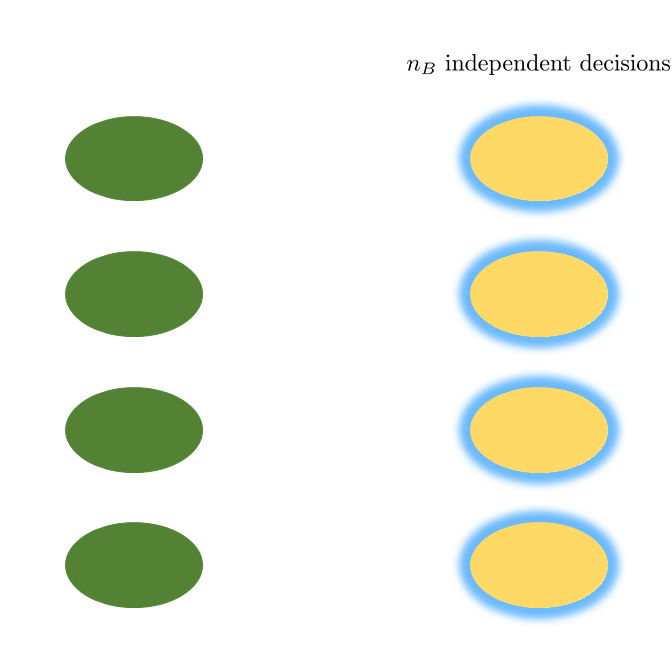
\includegraphics[width = \textwidth, height = .6\textwidth ]{graphics/Slide6.png}
%\end{frame}

\begin{frame}{Fellegi and Sunter (1969)}
	\begin{columns}
		\begin{column}{0.6\textwidth}
			\includegraphics<1>[width = \textwidth, height = 1.2\textwidth ]{graphics_square/Slide1.png}
			\includegraphics<2->[width = \textwidth, height = 1.2\textwidth ]{graphics_square/Slide2.png}
		\end{column}
		\begin{column}{0.38\textwidth}
			\begin{itemize}
				\item<3-> scalable to large datasets (\texttt{fastlink}, Enamorado et al 2019)
				\item<4-> not bipartite, requires post-processing
				\pause 
				\item<5-> overmatches, leading to inaccurate parameter estimation
			\end{itemize}

		\end{column}
	\end{columns}
\end{frame}

\begin{frame}{Sadinle (2017)}
	\begin{columns}
		\begin{column}{0.6\textwidth}
			\includegraphics<1>[width = \textwidth, height = 1.2\textwidth ]{graphics_square/Slide1.png}
			\includegraphics<2>[width = \textwidth, height = 1.2\textwidth ]{graphics_square/Slide3.png}
			\includegraphics<3>[width = \textwidth, height = 1.2\textwidth ]{graphics_square/Slide4.png}
			\includegraphics<4->[width = \textwidth, height = 1.2\textwidth ]{graphics_square/Slide5.png}
		\end{column}
		\begin{column}{0.38\textwidth}
			\begin{itemize}
				\item<1-> Beta Record Linkage (\texttt{BRL})
				\pause
				\item<5-> strictly enforces one-to-one matching, no post-processing
				\pause
				\item<6-> high accuracy for linkage and other parameters
				\pause 
				\item<7-> inherently serial, not scalable to large linkage tasks
			\end{itemize}
			
		\end{column}
	\end{columns}
\end{frame}

\begin{frame}{Our Contribution - Fast Beta Linkage}
	\begin{columns}
		\begin{column}{0.6\textwidth}
			\includegraphics<1>[width = \textwidth, height = 1.2\textwidth ]{graphics_square/Slide1.png}
			\includegraphics<2-4>[width = \textwidth, height = 1.2\textwidth ]{graphics_square/Slide6.png}
			\includegraphics<5>[width = \textwidth, height = 1.2\textwidth ]{graphics_square/Slide7.png}
			\includegraphics<6>[width = \textwidth, height = 1.2\textwidth ]{graphics_square/Slide8.png}
		\end{column}
		\begin{column}{0.38\textwidth}
			\begin{itemize}
				\item<3-> relaxation proposed by Heck Wortman (2019)
				\item<4-> minimal loss of accuracy, large computational gains
				\item<5-> allows for "one to many" matchings
				\item<6-> simple postprocessing to obtain bipartite matching
			\end{itemize}
			
		\end{column}
	\end{columns}
\end{frame}

\section{Fast Beta Linkage}
%\begin{frame}{Notation}
%\begin{itemize}
%	\item File A with records indexed $i \in \{1, \ldots, n_A\}$ and file B with records $j \in \{1, \ldots, n_B\}$, with $n_A \geq n_B$. We use $F$ features for linkage, with $L_f$ possible levels of agreement on feature $f$.
%	
%	\item $\Gamma \in \mathbb{R}^{n_A n_B \times F}$ matrix of comparison vectors where $\gamma_{ij}^f \in \{1, \ldots, L_f\}$
%	
%	\item $Z_j = \begin{cases} 
%	i,  & \text{if records } i\in A \text{ and } j\in B \text{ match}; \\
%	n_A + 1,  & \text{if record } j\in B \text{ has no match in } A; \\
%	\end{cases}$
%	
%	\item $m_{fl} = P\left(\gamma_{ij}^f = l |Z_j = i\right)$
%	
%	\item $u_{fl} = P\left(\gamma_{ij}^f = l |Z_j \neq i\right)$
%	
%	\item $\lambda = P(Z_j \leq n_A)$
%\end{itemize}
%\end{frame}

\begin{frame}{Fast Beta Linkage (\texttt{fabl})}
	$$P(\Gamma|\mathbf{Z}, \mathbf{m}, \mathbf{u}) = \prod_{j=1}^{n_B}  \prod_{i=1}^{n_A}\left[ \prod_{f=1}^{F}\prod_{l=1}^{L_f} m_{fl}^{I(Z_j = i)}u_{fl}^{I(Z_j \neq i)}\right]^{I(\gamma_{ij}^f = l)}$$
	
	$$\mathbf{m_{f}} \sim \text{Dirichlet}(\alpha_{f1}, \ldots, \alpha_{fL_f})$$
	$$\mathbf{u_{f}} \sim \text{Dirichlet}(\beta_{f1}, \ldots, \beta_{fL_f})$$
	$$Z_j | \pi	\begin{cases} 
	\frac{\pi}{n_A}  & z_j \leq n_A; \\
	1-\pi &  z_j  = n_A + 1 \\
	\end{cases}$$
	$$\pi \sim \text{Beta}(\alpha_{\pi}, \beta_{\pi})$$
	
	Note: the first three lines are common to many record linkage models, and bear similarities to a larger family of \textit{latent class models.} The last two lines are the newly developed prior distribution for the set of matches.  
\end{frame}

%\begin{frame}{Hashing}
%		\begin{columns}
%		\begin{column}{0.6\textwidth}
%			\begin{itemize}
%				\item<1-> Recognize there are at most $P = \prod_{f = 1}^F L_f$ unique agreement patterns, regardless of number of records (Enamorado et al 2019).
%				\begin{itemize}
%					\item<2-> $L = \{3, 3, 2, 2\}$ implies 36 unique patterns 
%				\end{itemize} 
%				\item<3-> When $(i,j)$ pair exhibits agreement pattern $p$, say $(i, j) \in h_p.$
%				\item<4-> Allows us to compute sufficient statistics and reduce computational complexity from $O(n_A \times n_B)$ to $O(P \times n_B)$
%			\end{itemize}
%		\end{column}
%		\begin{column}{0.38\textwidth}
%			\includegraphics<2->[width = \textwidth, height = 1.2\textwidth ]{graphics/unique_patterns.png}
%		\end{column}
%	\end{columns}
%\end{frame}
%
%\begin{frame}{Hashing}
%	\centering
%	\includegraphics<1>[width = 1.1\textwidth, height = .6\textwidth ]{graphics/Slide17.png}
%	\includegraphics<2>[width = 1.1\textwidth, height = .6\textwidth ]{graphics/Slide18.png}
%	\includegraphics<3>[width = 1.1\textwidth, height = .6\textwidth ]{graphics/Slide19.png}
%	\includegraphics<4>[width = 1.1\textwidth, height = .6\textwidth ]{graphics/Slide20.png}
%	\includegraphics<5>[width = 1.1\textwidth, height = .6\textwidth ]{graphics/Slide21.png}	
%\end{frame}
%
%\begin{frame}{Hashing to Scale to Large Linkage Tasks}
%	\includegraphics<1>[width = \textwidth, height = .6\textwidth ]{graphics/Slide23.png}
%	\includegraphics<2>[width = \textwidth, height = .6\textwidth ]{graphics/Slide24.png}
%	\includegraphics<3>[width = \textwidth, height = .6\textwidth ]{graphics/Slide25.png}
%	\includegraphics<4>[width = \textwidth, height = .6\textwidth ]{graphics/Slide26.png}
%	\includegraphics<5>[width = \textwidth, height = .6\textwidth ]{graphics/Slide27.png}
%\end{frame}
%
%\begin{frame}{Hashing for Speed (Efficient Gibbs Sampling)}
%	\includegraphics<1>[width = \textwidth, height = .6\textwidth ]{graphics/Slide37.png}
%	\includegraphics<2>[width = \textwidth, height = .6\textwidth ]{graphics/Slide38.png}
%	\includegraphics<3>[width = \textwidth, height = .6\textwidth ]{graphics/Slide39.png}
%	\includegraphics<4>[width = \textwidth, height = .6\textwidth ]{graphics/Slide40.png}
%	\includegraphics<5>[width = \textwidth, height = .6\textwidth ]{graphics/Slide41.png}
%	\includegraphics<6>[width = \textwidth, height = .6\textwidth ]{graphics/Slide42.png}
%\end{frame}



%\begin{frame}{Managing Large Data}
%	\begin{itemize}
%		\item \textbf{Distributed Computing} - Partition data in to chunks $\{A_I\}$ and $\{B_J\}$. Compare records, hash results, compute summary statistics in parallel, and synthesize results.
%		
%		\item \textbf{Storage Efficient Indexing (SEI)} - Store at most small number $R$ many record labels in each $r_{p_j}$, remove highly unlikely record labels from memory. Proper weights for calculations maintained through summary statistics $\{H_p\}$ and $\{H_{p_j}\}$.
%		
%		\item Hashing plus SEI can reduce memory requirements by $>99$.
%		\begin{itemize}
%			\item Simulation of $20,000 \times 20,000$ linkage task with 4 fields. Naive approach requires 6.4GB of storage for all-to-all comparisons, hashing and SEI requires 90MB.
%		\end{itemize}
%	\end{itemize}
%\end{frame}

\section{Simulation Studies}

%\begin{frame}{Three Simulation Studies}
%	\begin{itemize}
%		\item We compare \texttt{fabl} against \texttt{BRL} in three simulation studies
%		\begin{itemize}
%			\item Measure precision and recall on 100 simulated datasets and varying levels of error and duplication across files
%			\item Measure speed when both $n_A$ and $n_B$ are increasing
%			\item Measure speed when $n_A$ is increasing and $n_B = 500$ is fixed. 
%		\end{itemize}
%	\end{itemize}
%\end{frame}

\begin{frame}{Speed Simulation 1}
	\begin{columns}
		\begin{column}{0.38\textwidth}
			\begin{itemize}
				\item $F$ = 5 comparison fields
				\item L = \{2, 2, 2, 2, 2\}, all binary comparisons
				\item 32 possible patterns
				\item Increase both $n_A$ and $n_B$
			\end{itemize}
		\end{column}
		\begin{column}{0.58\textwidth}
			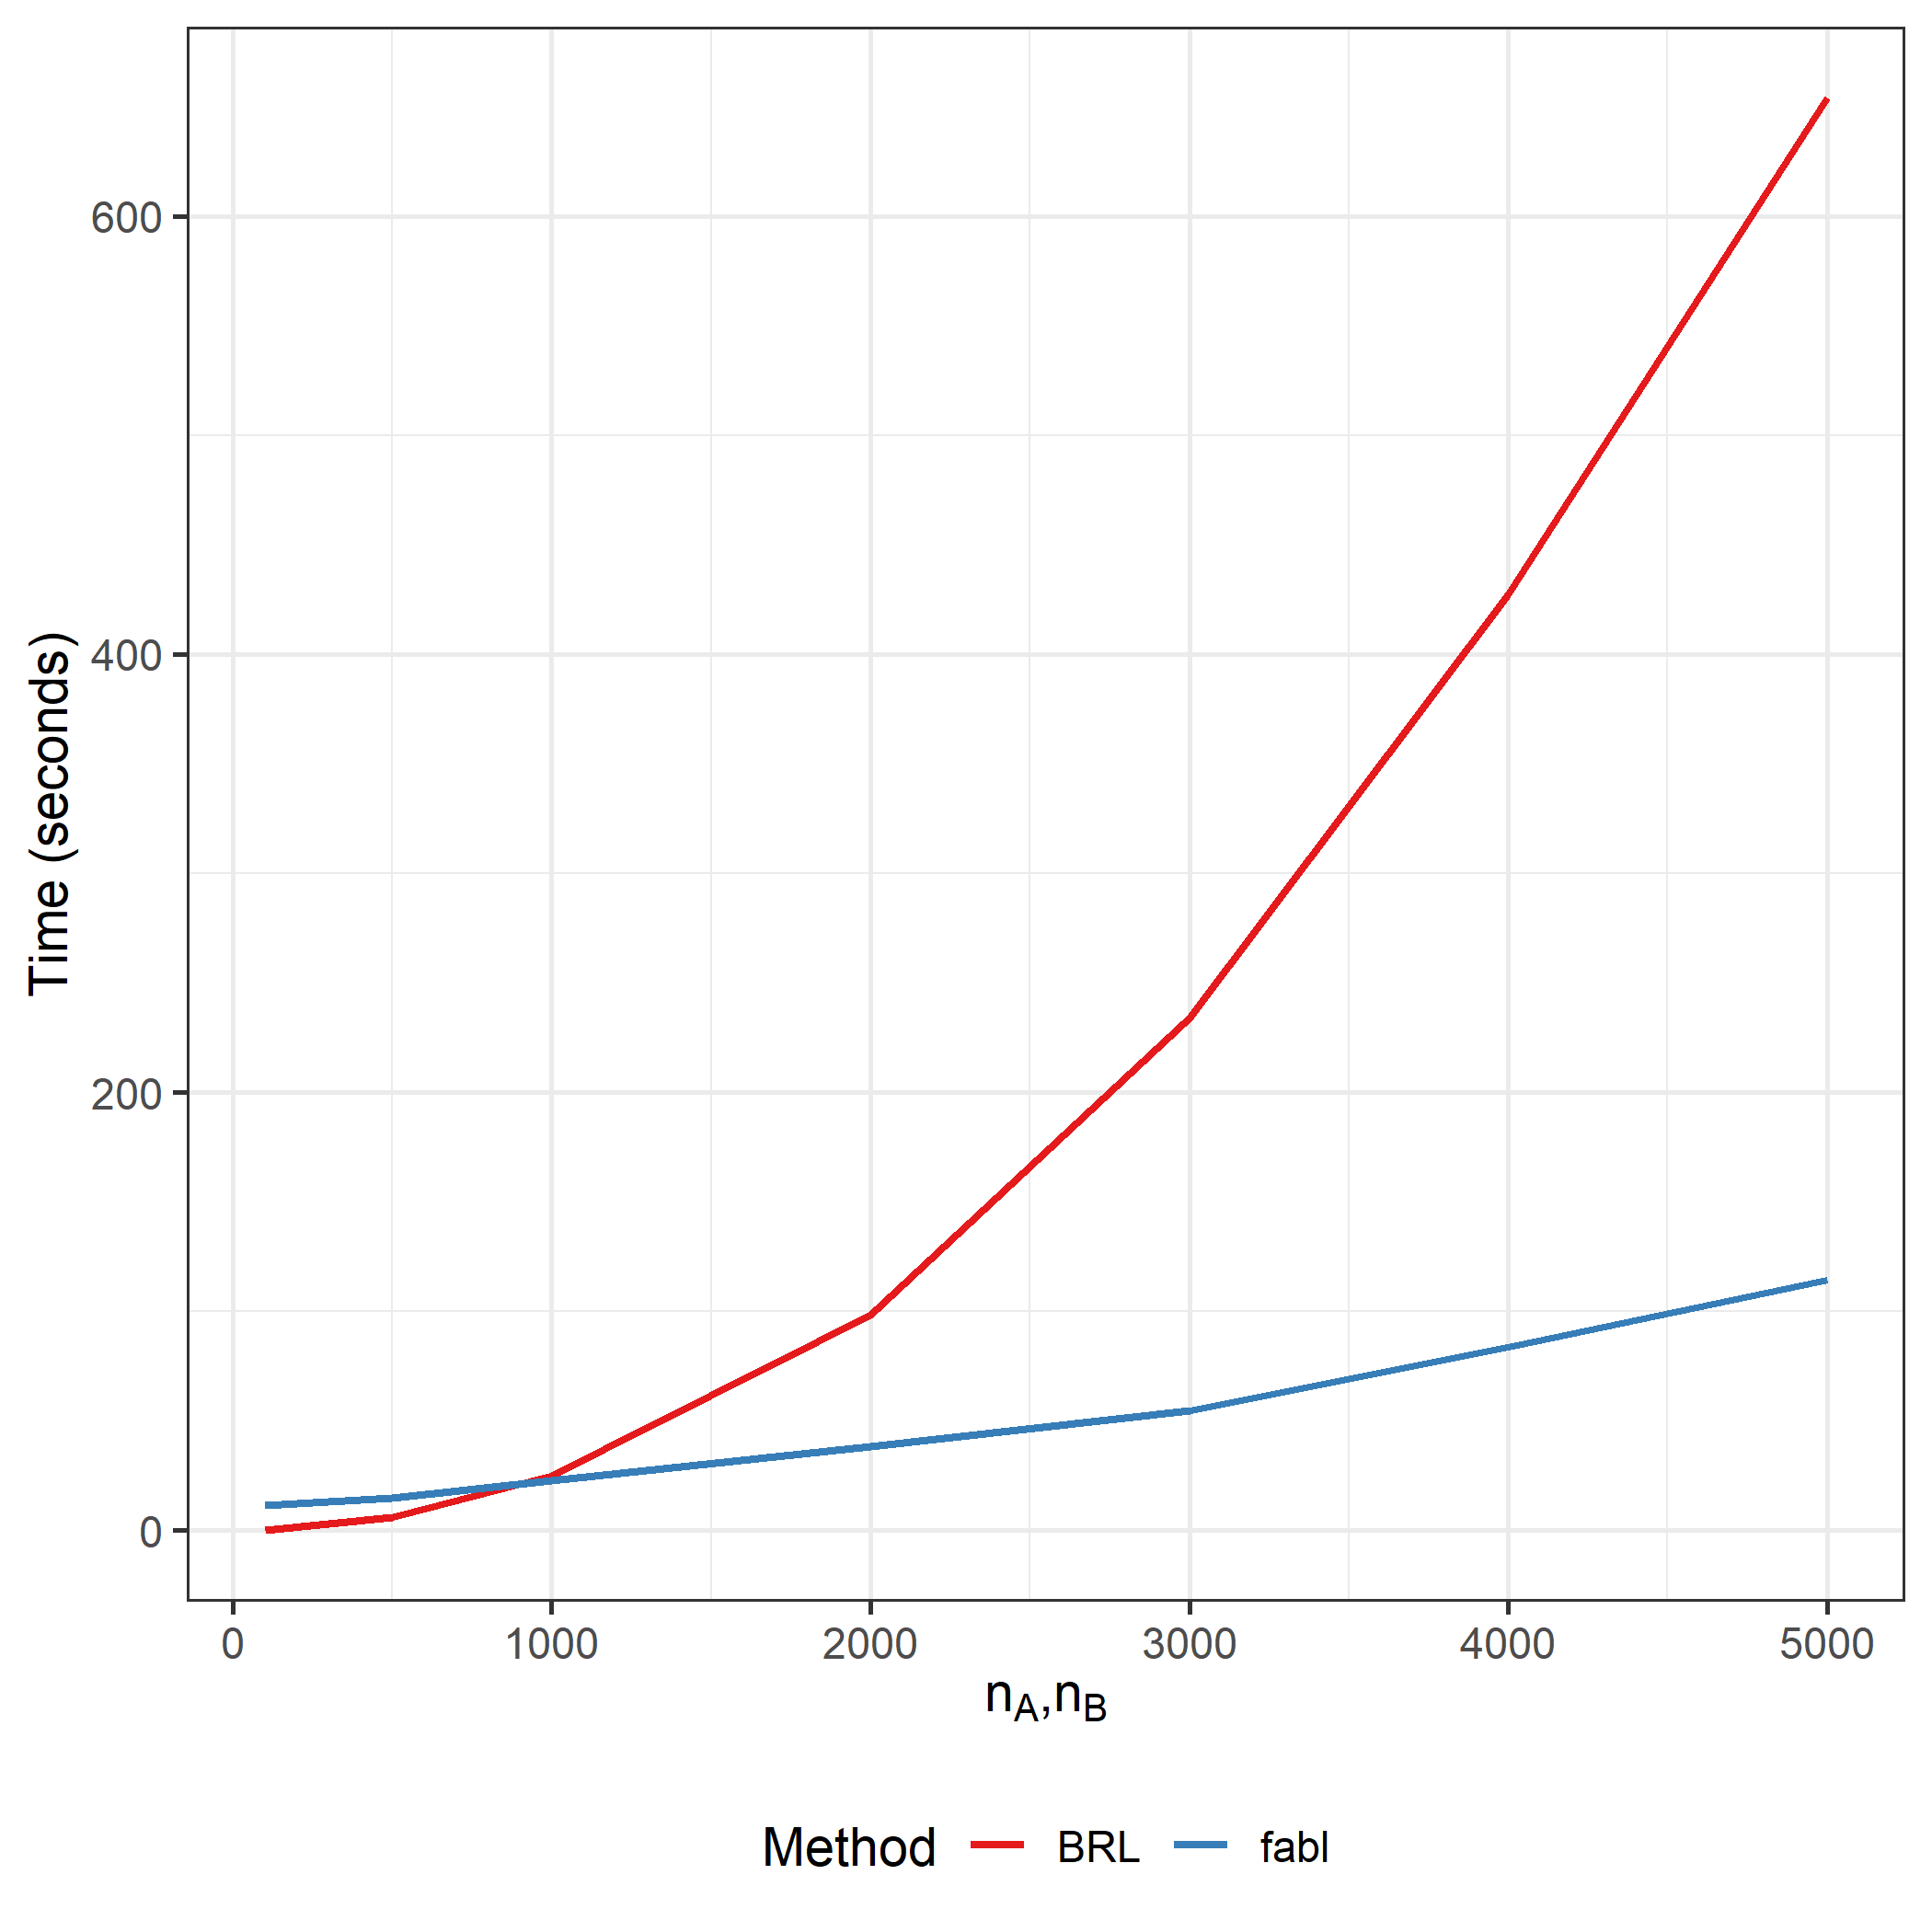
\includegraphics[width = \textwidth, height = \textwidth ]{../notes/figures/sadinle_speed_plot_slides.png}
		\end{column}
	\end{columns}
\end{frame}

\begin{frame}{Speed Simulation 2}
	\begin{columns}
		\begin{column}{0.38\textwidth}
			\begin{itemize}
				\item $F$ = 5 comparison fields
				\item L = \{2, 2, 2, 2, 2\}, all binary comparisons
				\item 32 possible patterns
				\item Fix $n_B = 500$, increase $n_A$
			\end{itemize}
		\end{column}
		\begin{column}{0.58\textwidth}
			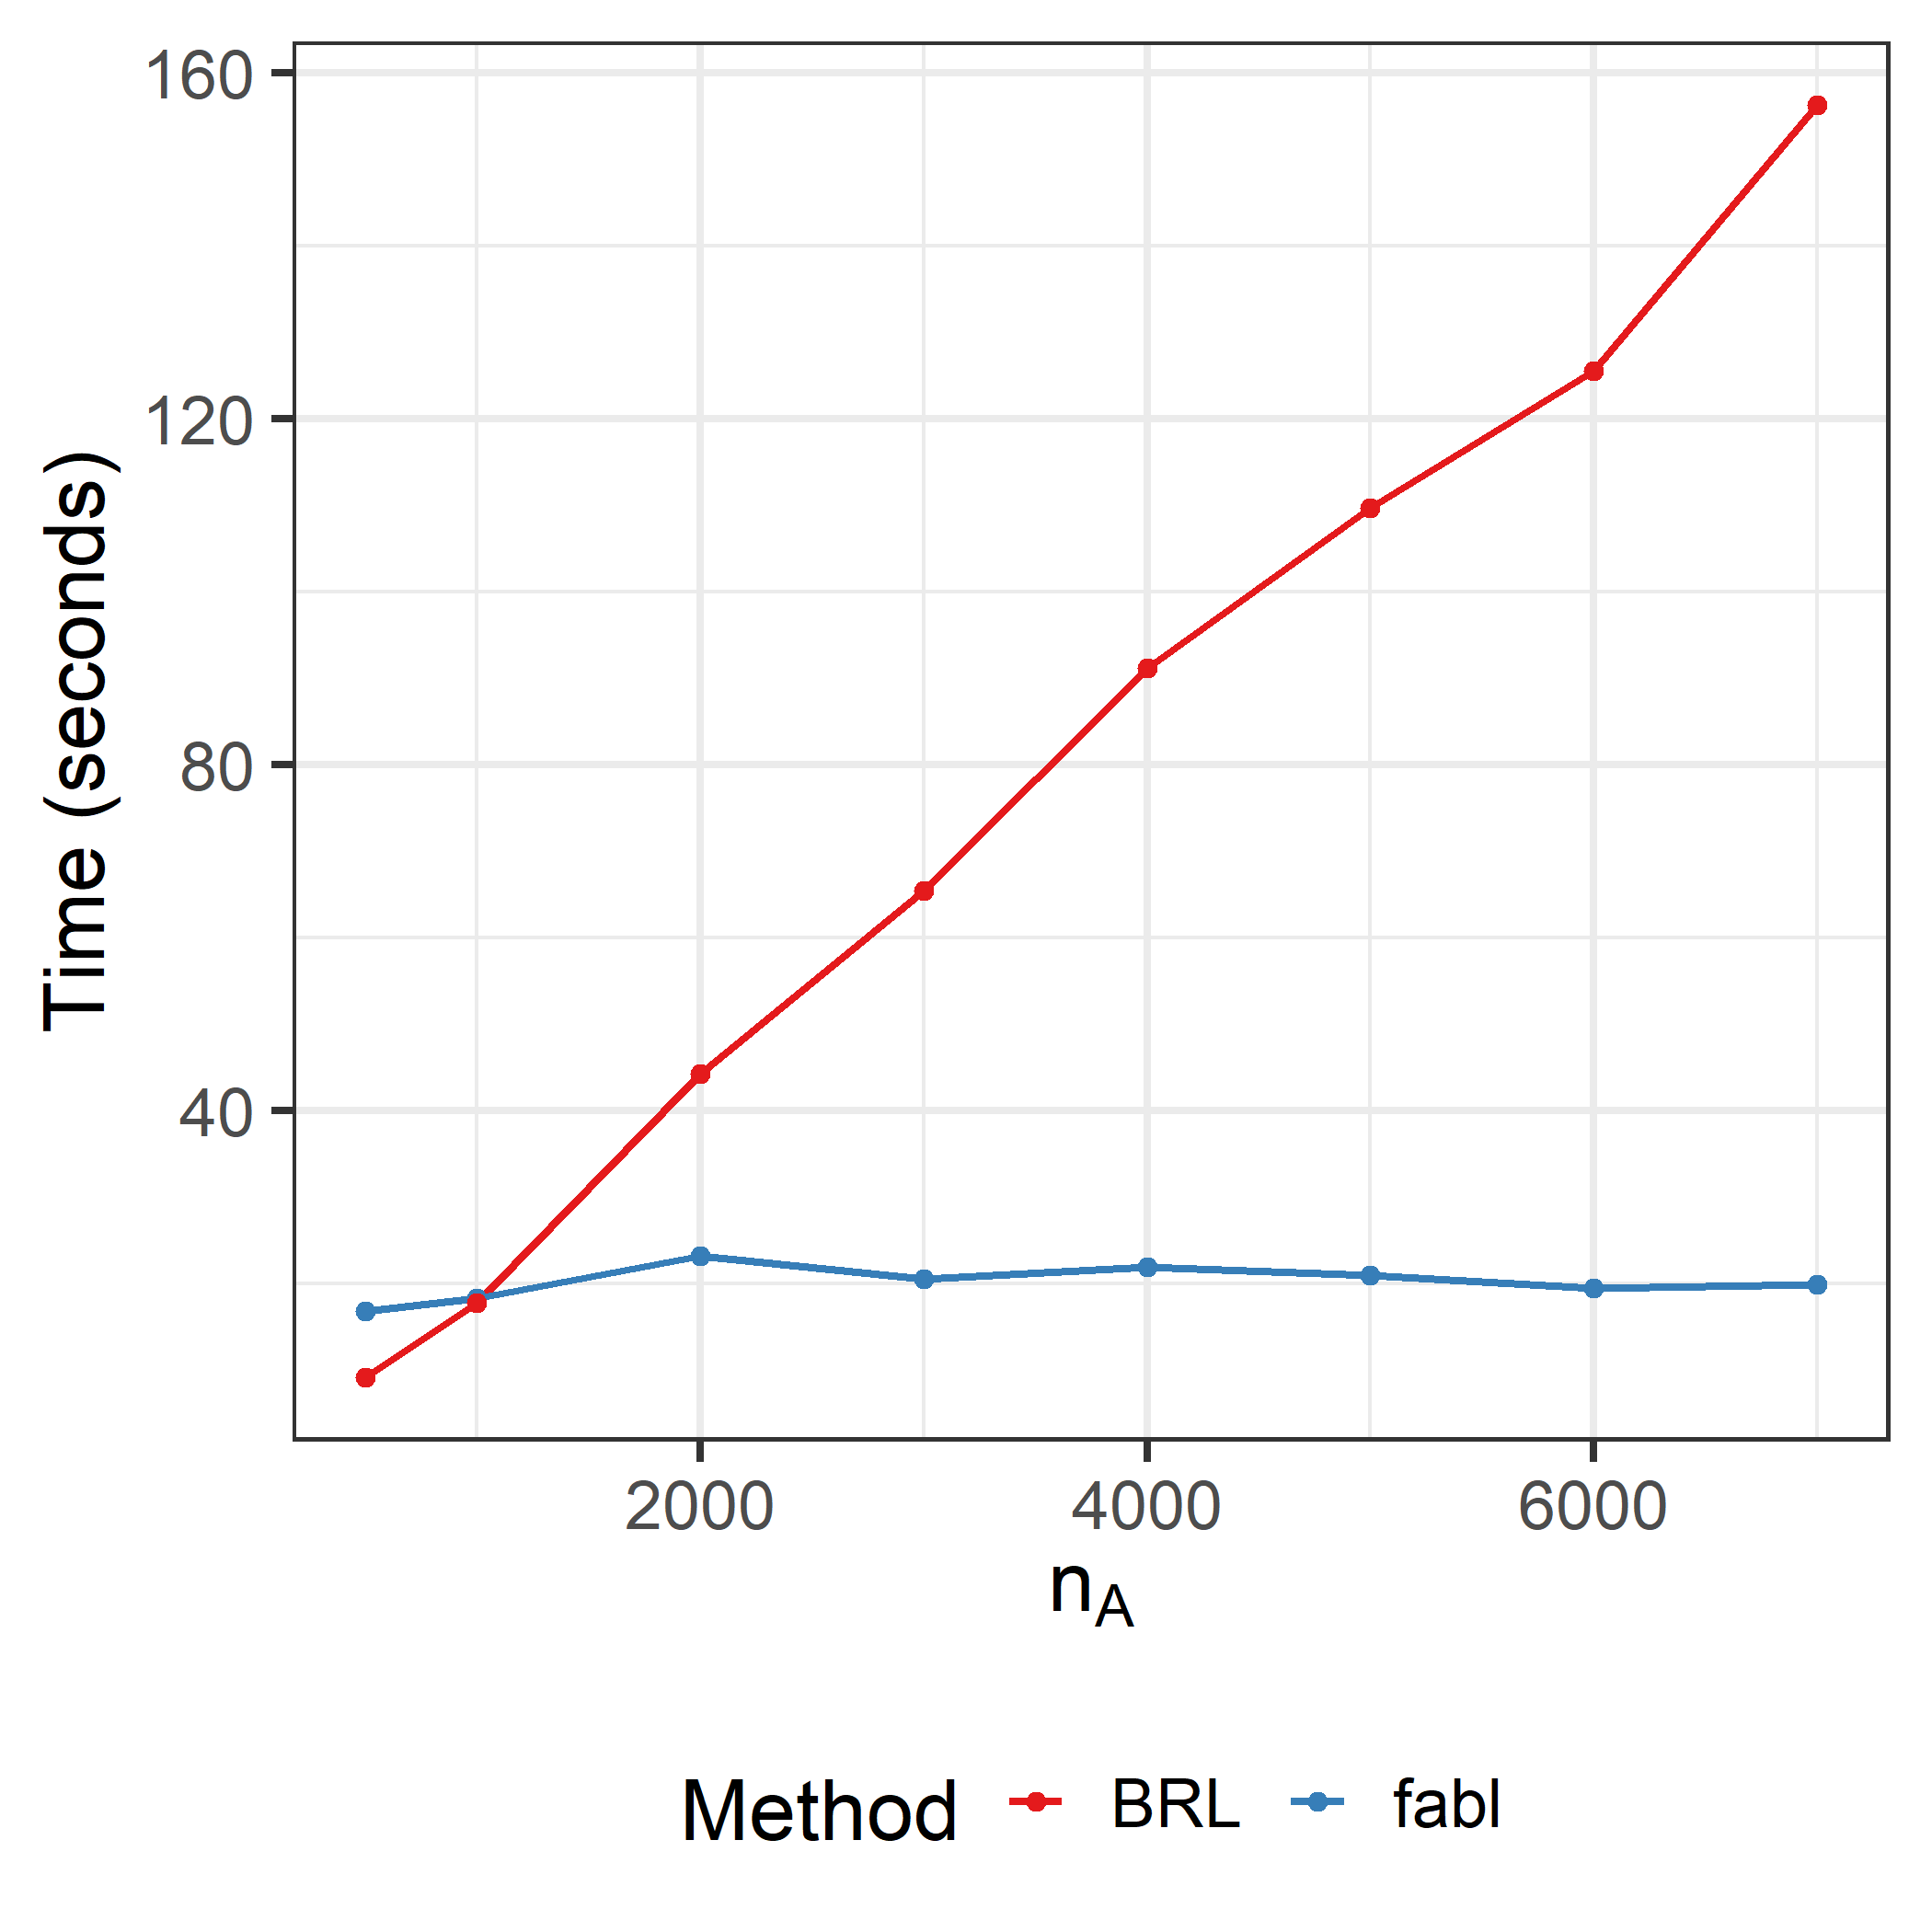
\includegraphics[width = \textwidth, height = \textwidth ]{../notes/figures/speed_plot_fixed_nB_slides.png}
		\end{column}
	\end{columns}
\end{frame}

\begin{frame}{Accuracy Simulation}
	\begin{itemize}
		\item Sadinle (2017) used 900 simulated linkage tasks to show accuracy of \texttt{BRL}
		\item Find matches across two datasets, each with 500 records and 4 fields in common. 
		\item One, two or three errors across matching records
		\item 10\% matching, 50\% matching, or 90\% matching
		\item Calculate recall, precision, and F-measure 
	\end{itemize}
\end{frame}

\begin{frame}{Accuracy Simulation}
	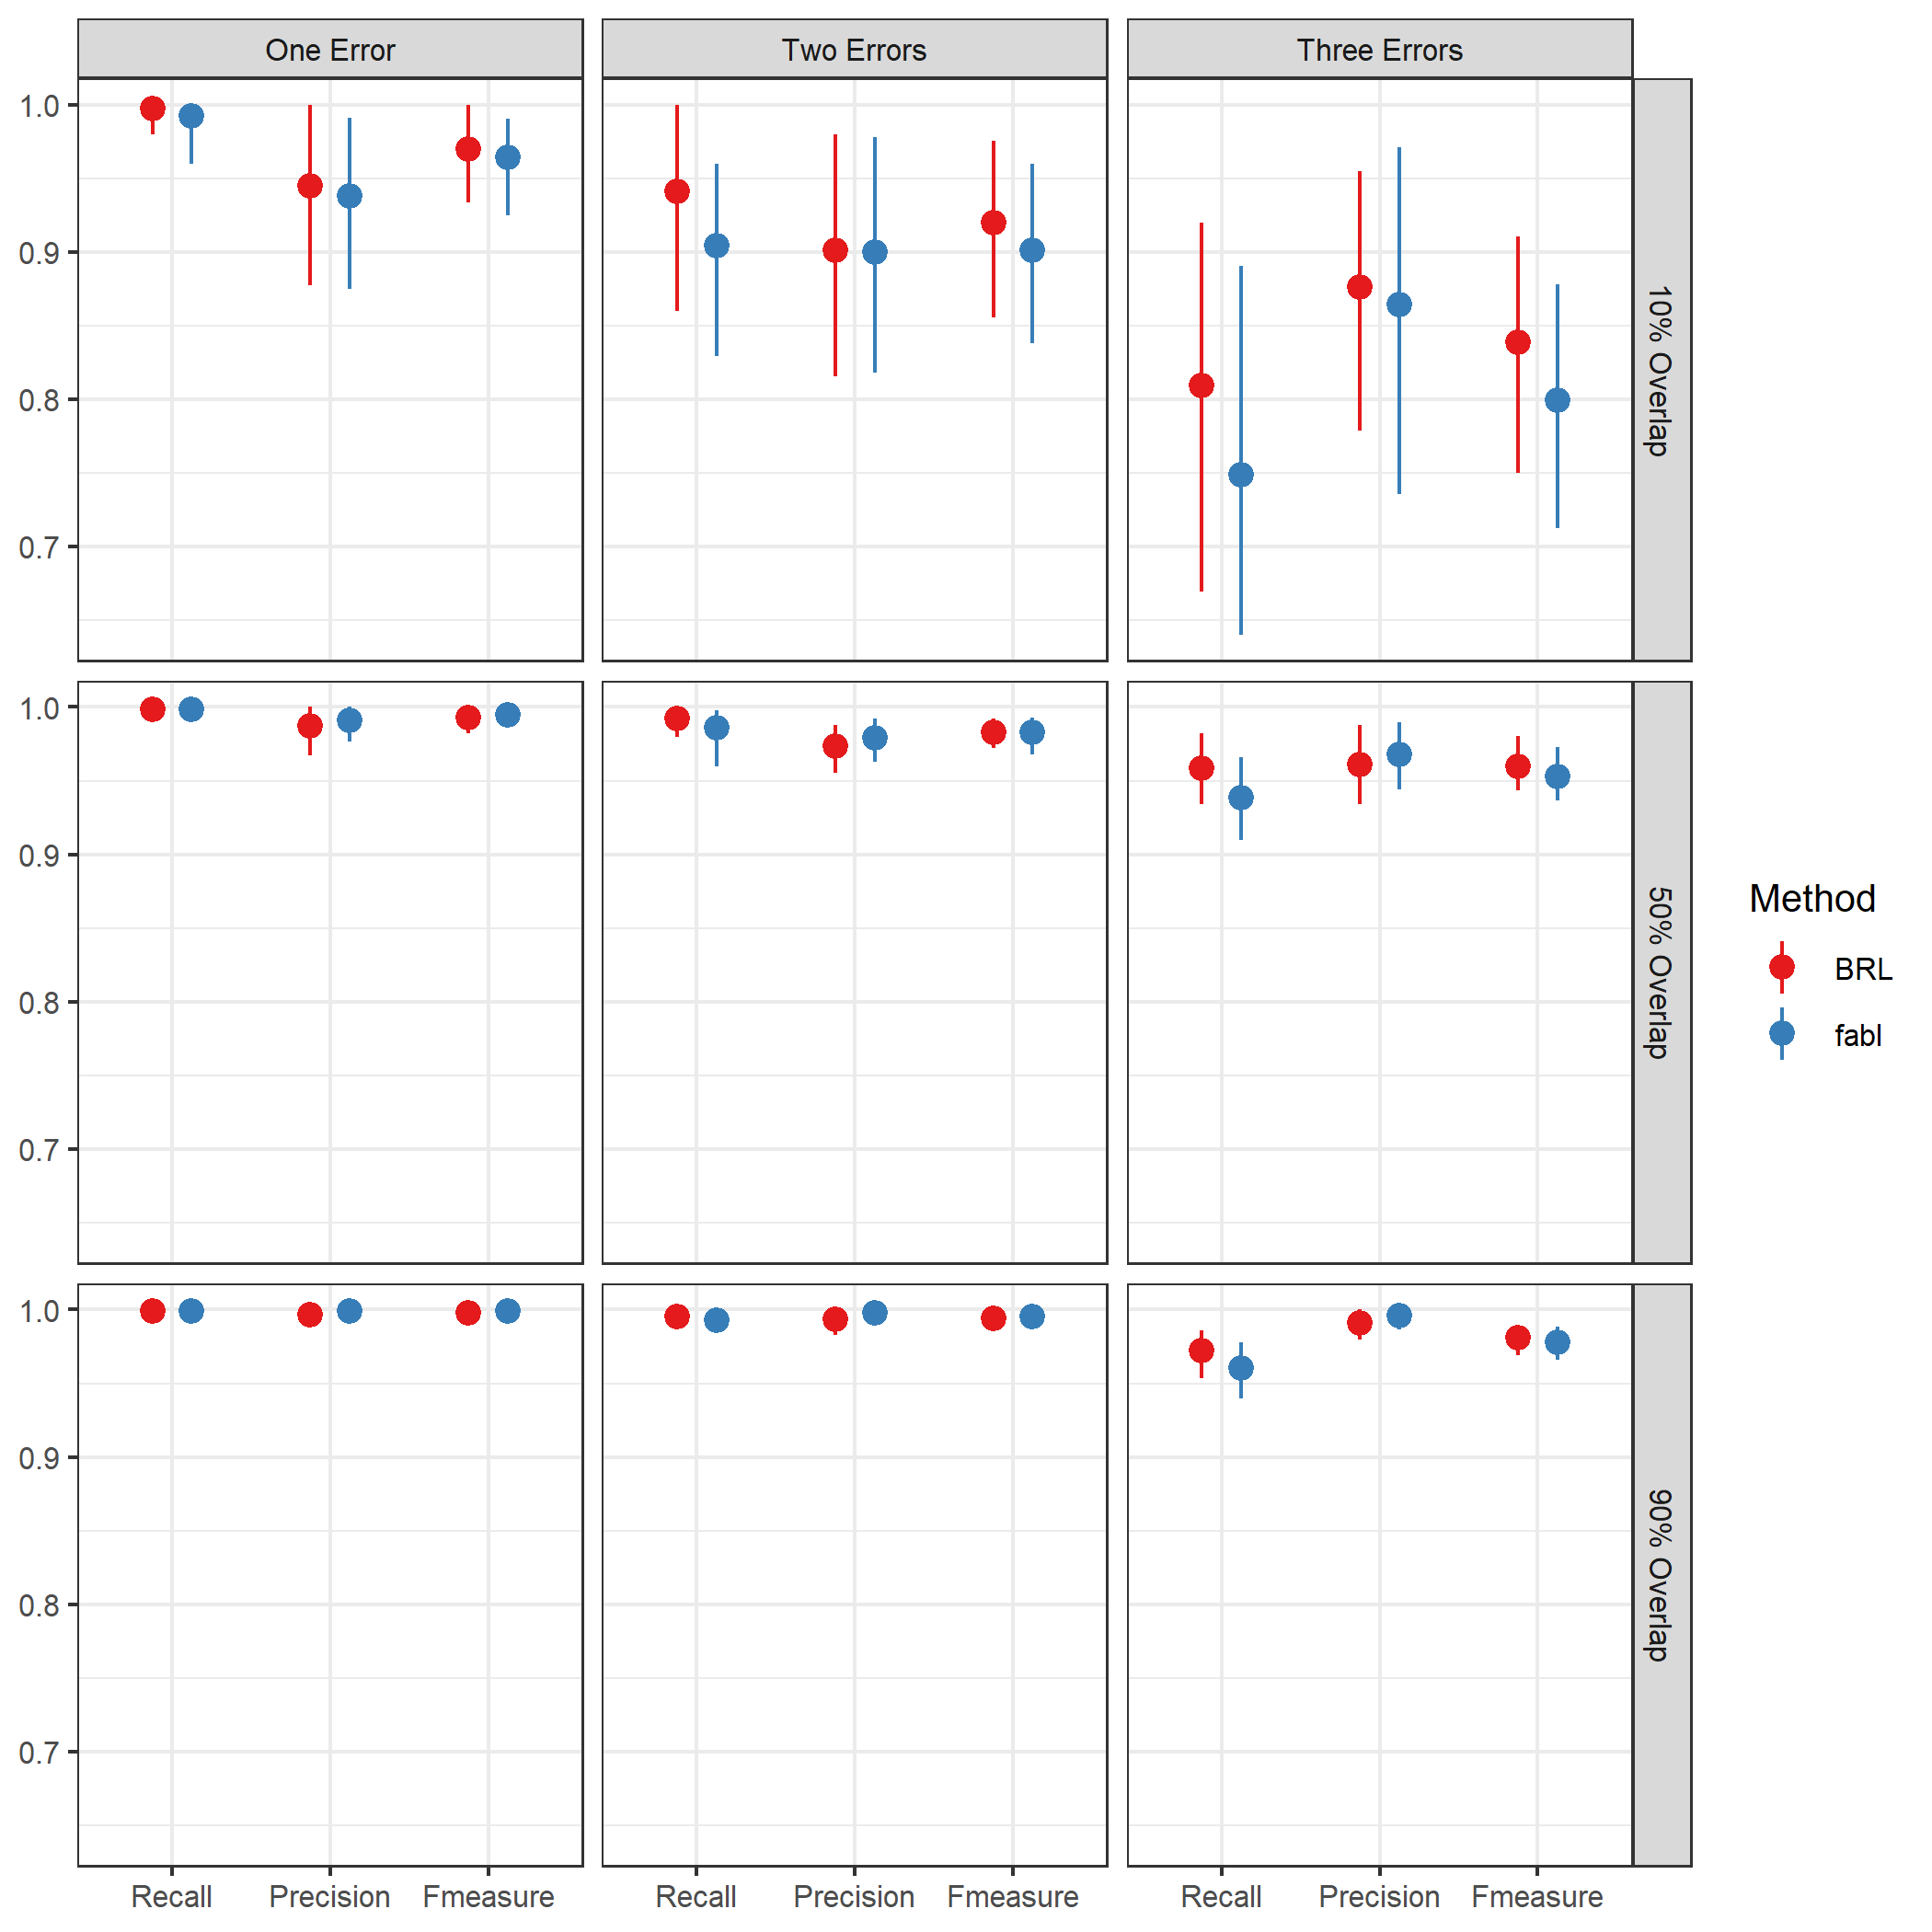
\includegraphics[width = \textwidth, height = .7\textwidth ]{../notes/figures/sadinle_sim_plot2.png}
\end{frame}

%\begin{frame}{Speed Simulation 1}
%	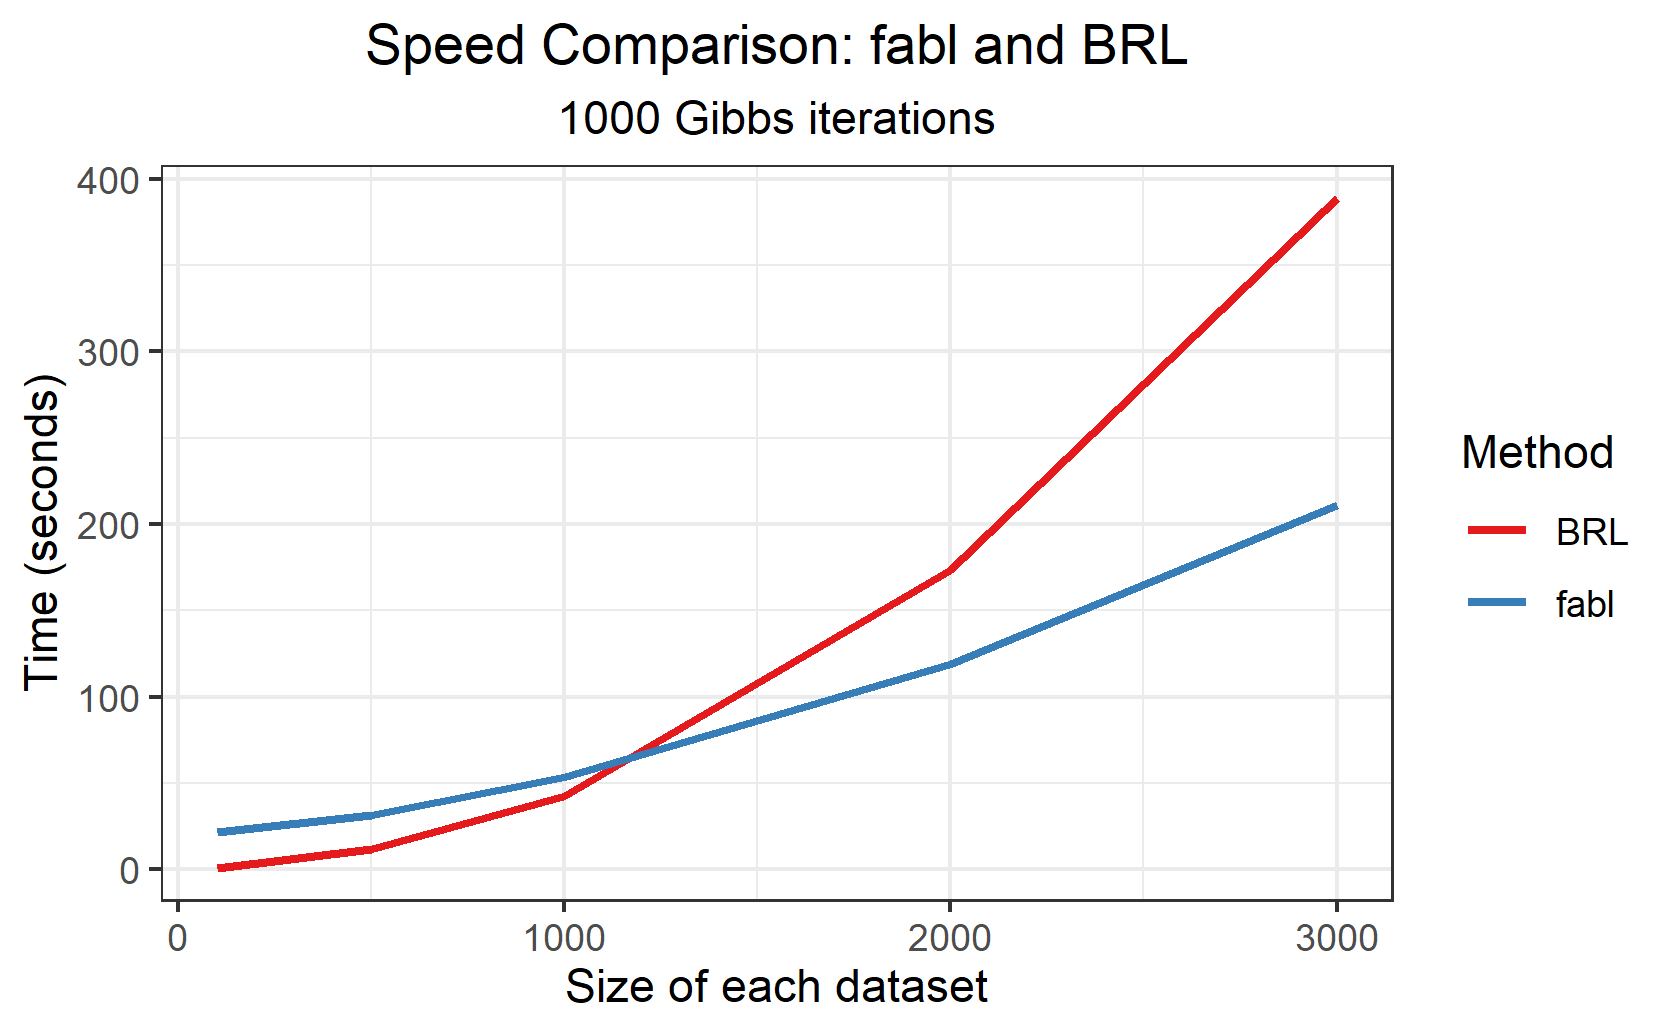
\includegraphics[width = \textwidth, height = .7\textwidth ]{../notes/figures/sadinle_speed_plot2.png}
%\end{frame}
%
%	\begin{frame}{Speed Simulation 2}
%	
\includegraphics[width = \textwidth, height = .7\textwidth ]{../notes/figures/speed_plot_fixed_nB.png}
%\end{frame}



%\section{El Salvador Homicide Case Study}
%
%\begin{frame}{El Salvador Case Study}
%	\begin{itemize}
%		\item El Salvadoran Civil War (1980-1991)
%		\item Lists of casualties collected by multiple organizations
%		\begin{itemize}
%			\item Salvadoran Human Rights Commissions (CDHES), $n_A = 4420$
%			\item El Rescate - Tutela Regal (ERTL), $n_B = 1323$
%			\item Features include first name, last name, date and place of death
%		\end{itemize}
%		\item We aim to find duplicate records across files
%		\begin{itemize}
%			\item Particularly difficult because families are often killed together, and some children share names with parents
%		\end{itemize}
%
%	\end{itemize}
%\end{frame}
%
%\begin{frame}{Run Time}
%		\begin{columns}
%		\begin{column}{0.48\textwidth}
%			\centering
%			\includegraphics<1->[width = .6\textwidth, height = .6\textwidth ]{../notes/figures/el_salvador/time_table_big_P2.png}
%			
%		\end{column}
%		\begin{column}{0.48\textwidth}
%			\centering
%			\includegraphics<2>[width = .6\textwidth, height = .6\textwidth ]{../notes/figures/el_salvador/time_table_small_P2.png}	
%		\end{column}
%	\end{columns}
%\end{frame}
%
%\begin{frame}{Posterior Inference}
%	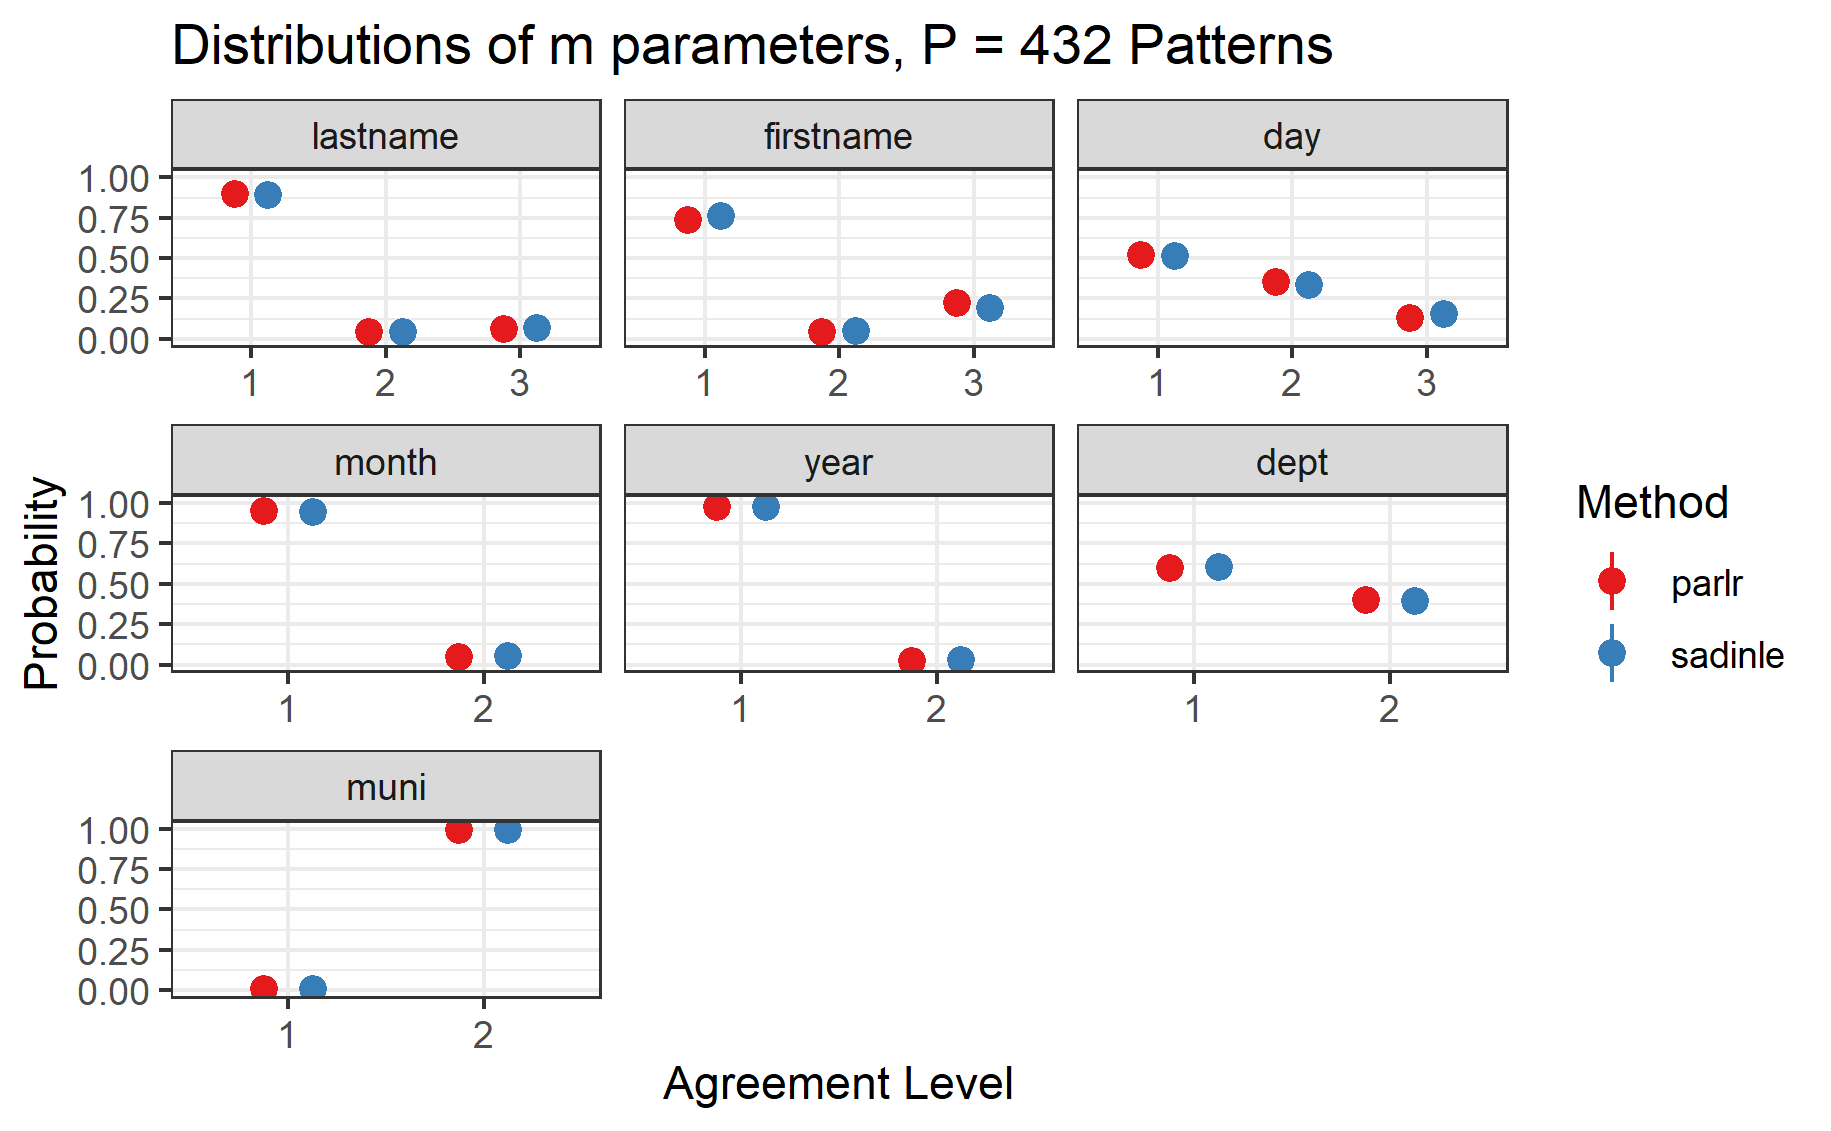
\includegraphics[width = \textwidth, height = .6\textwidth ]{../notes/figures/el_salvador/m_posterior_smallP.png}
%\end{frame}
%
%\begin{frame}{Posterior Inference}
%	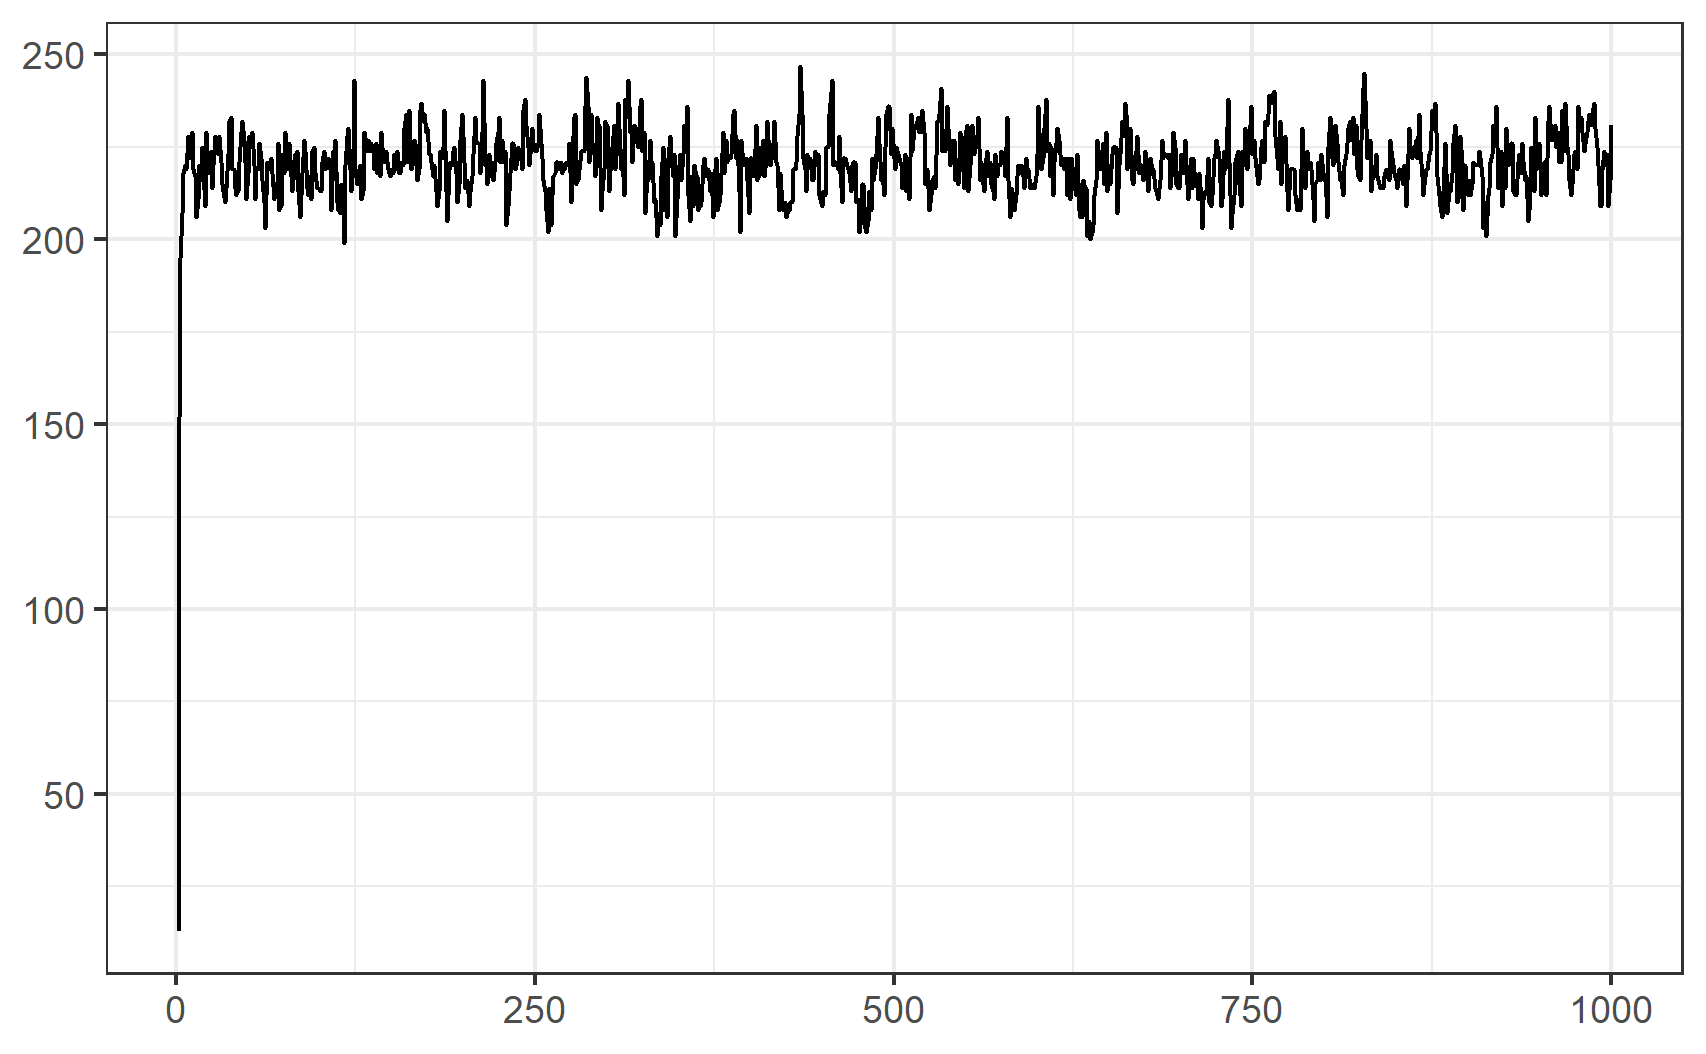
\includegraphics[width = \textwidth, height = .6\textwidth ]{../notes/figures/el_salvador/DID_distribution_smallP_bayes.png}
%\end{frame}
%
%\begin{frame}{Violations of One-to-One Matching}
%	\centering
%	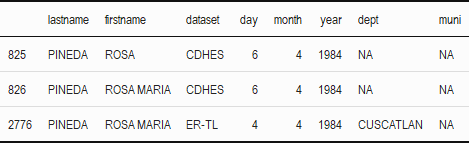
\includegraphics[width = .9\textwidth, height = .4\textwidth ]{../notes/figures/el_salvador/rosa_records.png}
%\end{frame}
%
%\begin{frame}{Violations of One-to-One Matching}
%	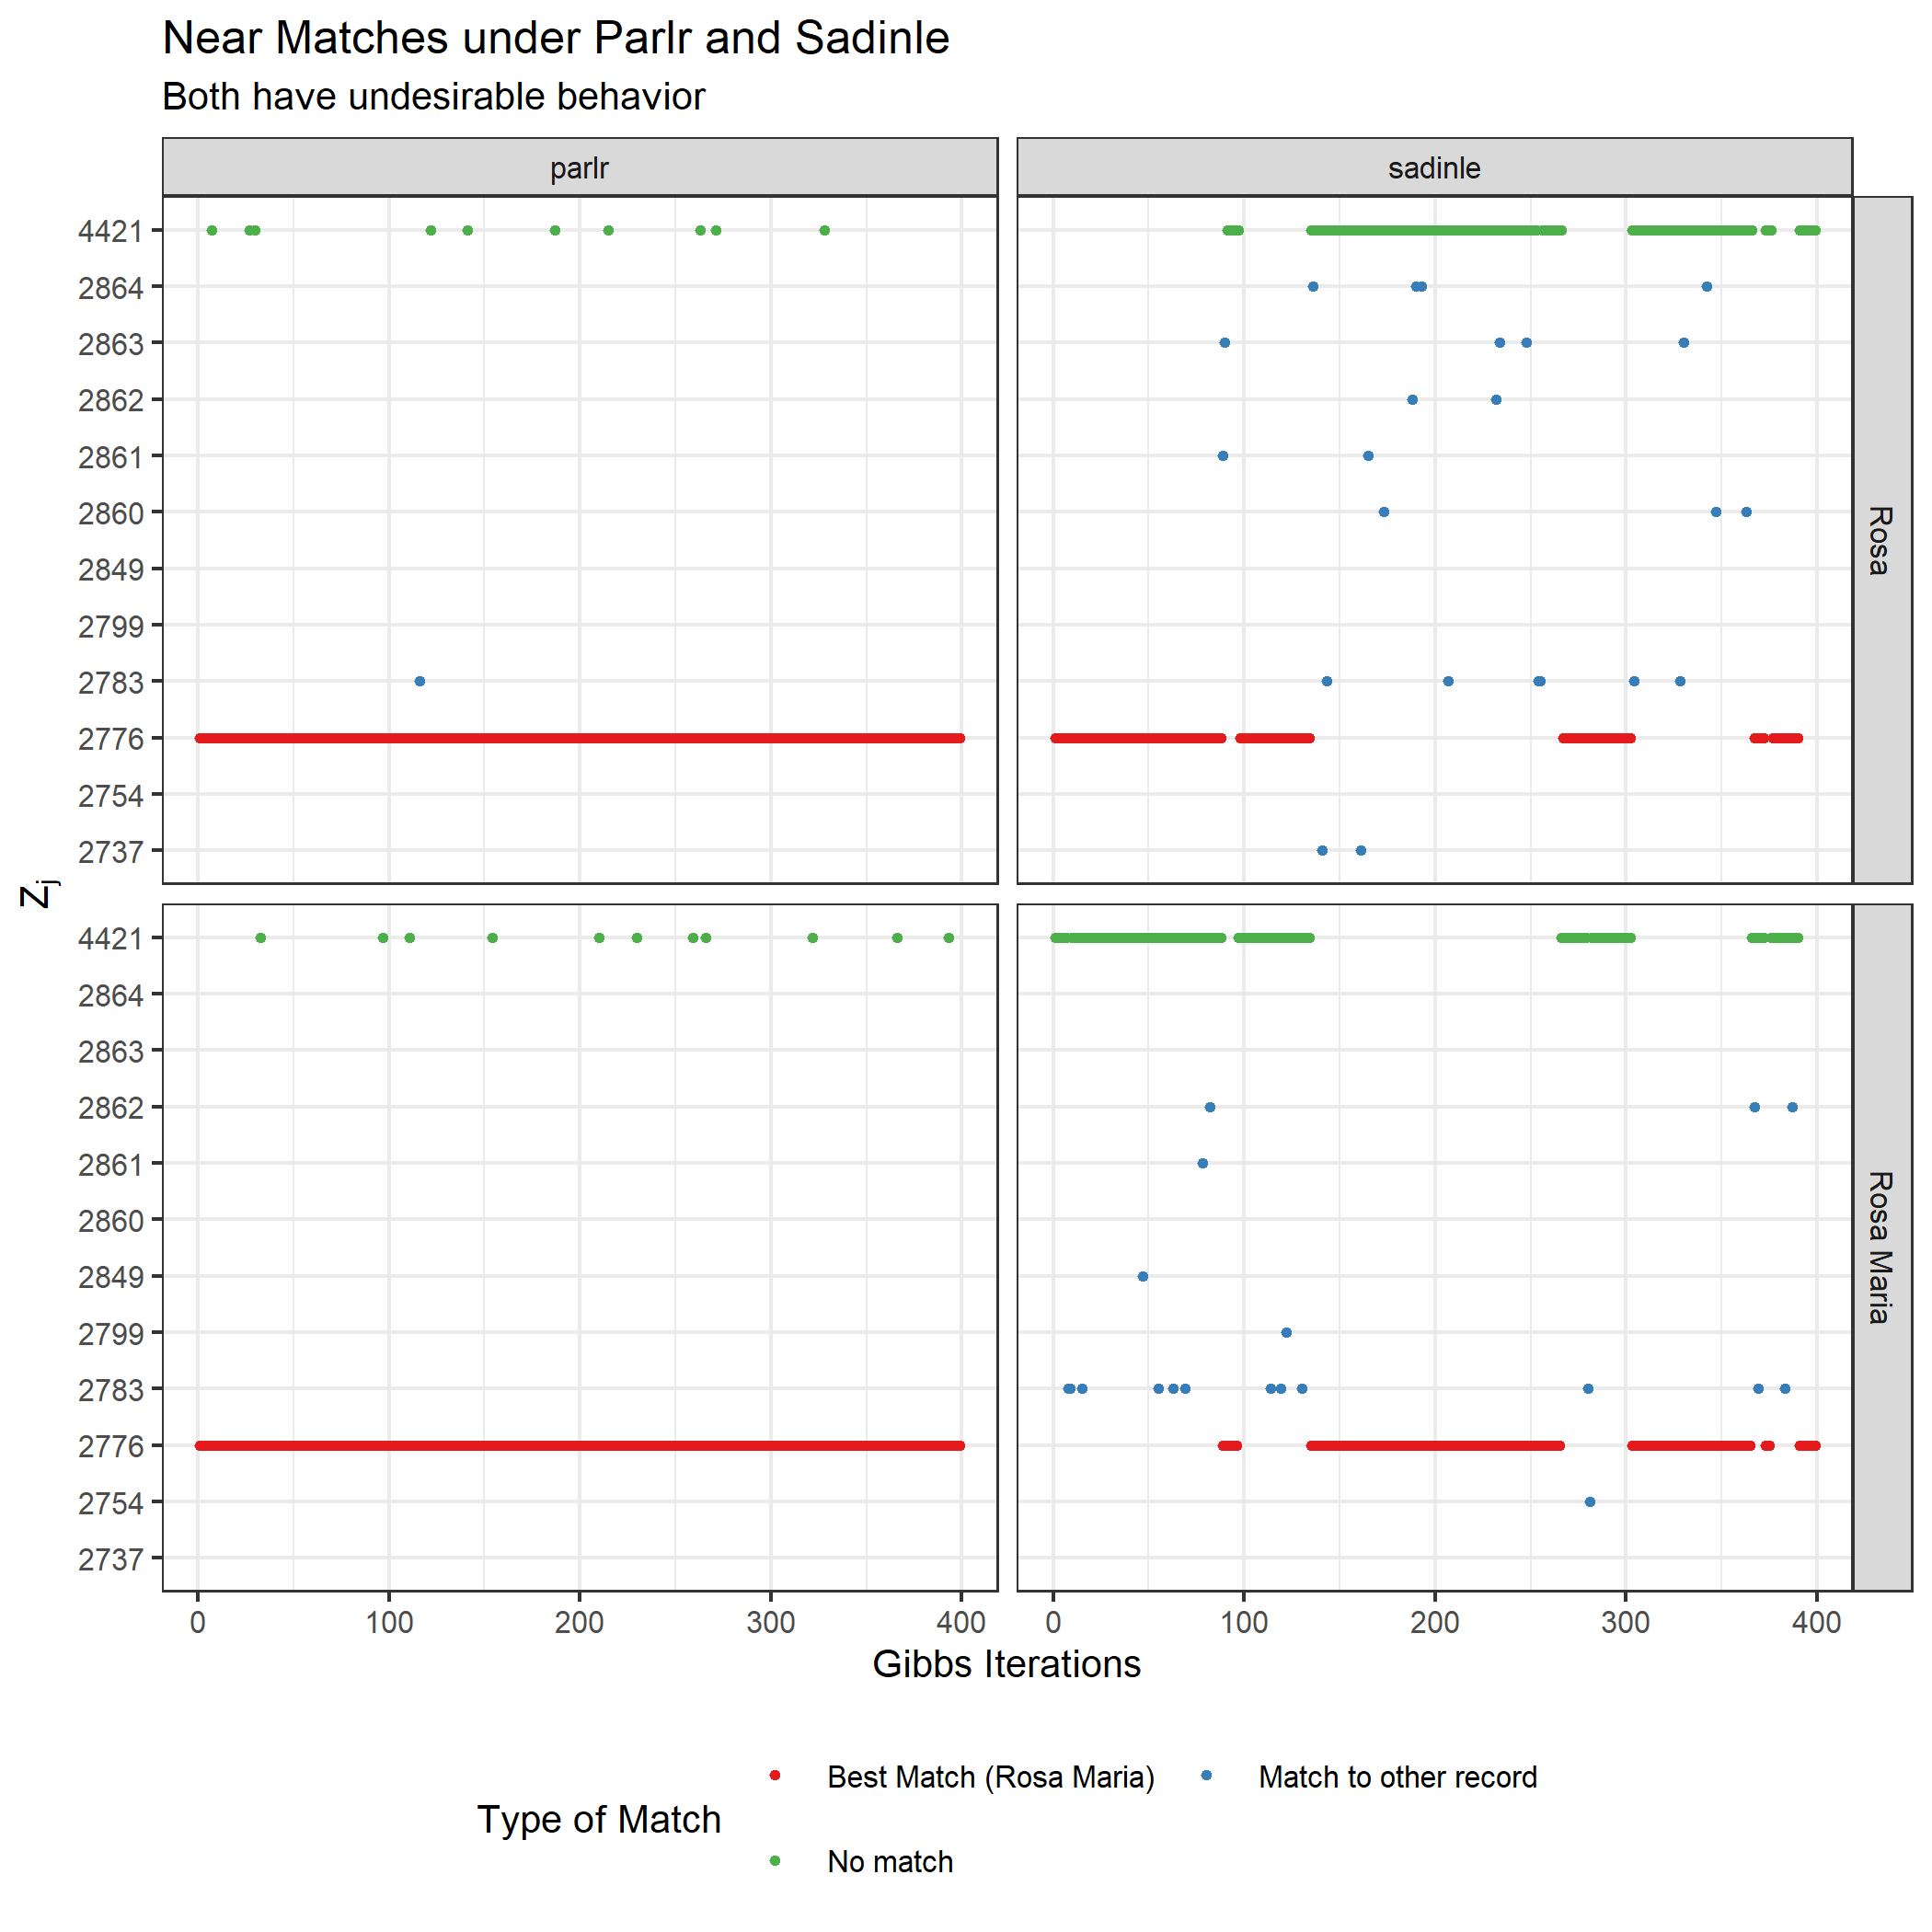
\includegraphics[width = \textwidth, height = .6\textwidth ]{../notes/figures/el_salvador/bad_mixing.png}
%\end{frame}
%


\section{Conclusion}

\begin{frame}{Benefits of \texttt{fabl}}
	\begin{itemize}
		\item Faster computation for larger linkage tasks
		
		\item Accurate estimation of linkage structure $\mathbf{Z}$, and additional parameters $\mathbf{m}$ and $\mathbf{u}$
		
		\item Bayesian model with natural uncertainty quantification
	\end{itemize}
\end{frame}

\begin{frame}{Glaring Questions}
	\begin{itemize}
		\item Can you do record linkage with arbitrary amounts of duplicated files?
		\begin{itemize}
			\item<2-> Yes! See Aleshin-Guendel and Sadinle (2021)
		\end{itemize}
		
		\item Isn't $n_A \times n_B$ record pairs computationally infeasible?
		\begin{itemize}
			\item<3-> Yes! My work with the DNC is forthcoming, Kundinger, Wortman, Reiter, and Steorts (2022)
		\end{itemize}
		
		\item Can you account situations when the reliability of information differs throughout the data?
		\begin{itemize}
			\item<4-> Yes! I have a heirarchical model in the works. Hopefully Kundinger et al (2023)
		\end{itemize}
		
		\item Can you do record linkage on the records themselves, rather than transforming to comparison vectors?
		\begin{itemize}
			\item<5-> Yes! See \texttt{d-blink} package from Marchant et al (2021)
		\end{itemize}
		
	\end{itemize}
\end{frame}


\section{Possible Relevance to Google}
\begin{frame}{Latent Class Analysis}
	The record linkage model presented is a special case of a "latent class model". In my work, we attempt to classify record pairs into two distinct classes: matching, and non-matching pairs.
	\linebreak 
	
	One can imagine however, that we can look at articles instead of records, look at blocks of text instead of record pairs, and look at attributes of those blocks instead of comparison vectors. This may provide a strategy for \textbf{entirely unsupervised} byline detection.
	\linebreak
	
	Additionally, if model parameters are accurate, we can train the model on a small set of articles, and then apply those parameters out onto a larger set of articles, for nearly instantaneous latent class analysis. 
\end{frame}


\end{document}